% Quadrat-grid figure — 6 representative test-set quadrats arranged 2×3.
% Each cell shows the quadrat photograph with its filename (which
% encodes the transect site + date) as a caption above.
%
% Required host preamble:
%   \usepackage{graphicx}
%   \usepackage{tikz}
%
% Images live in archive/report/images/quadrats/.

\begin{tikzpicture}[
  every node/.style={inner sep=0pt, outer sep=0pt},
  label/.style={font=\sffamily\tiny, text=black!70, align=center},
]

% Cell dimensions: 3 columns, 2 rows; ~5.4cm wide cells leaves slight gap
\def\cellw{52mm}
\def\cellh{52mm}
\def\colsep{2mm}
\def\rowsep{6mm}

% ── Row 1 ──────────────────────────────────────────────────────────────
\node[label]                              (l1) at (0,                              0)              {CBN-PdlC-A1-20130807.jpg};
\node[below=1mm of l1]                    (i1)                                                     {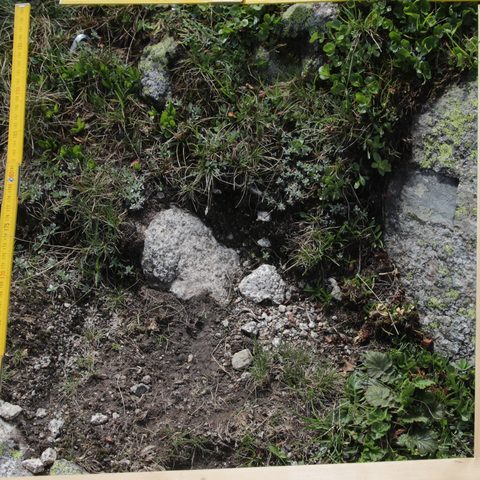
\includegraphics[width=\cellw, height=\cellh, keepaspectratio]{images/quadrats/CBN-PdlC-A1-20130807.jpg}};

\node[label, right=\colsep of l1.east, anchor=west] (l2) {CBN-Pla-A1-20130808.jpg};
\node[below=1mm of l2]                              (i2) {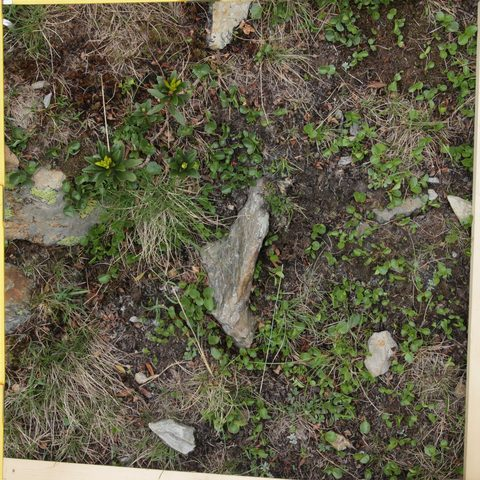
\includegraphics[width=\cellw, height=\cellh, keepaspectratio]{images/quadrats/CBN-Pla-A1-20130808.jpg}};

\node[label, right=\colsep of l2.east, anchor=west] (l3) {GUARDEN-CBNMed-10-1-16-34-20240429.jpg};
\node[below=1mm of l3]                              (i3) {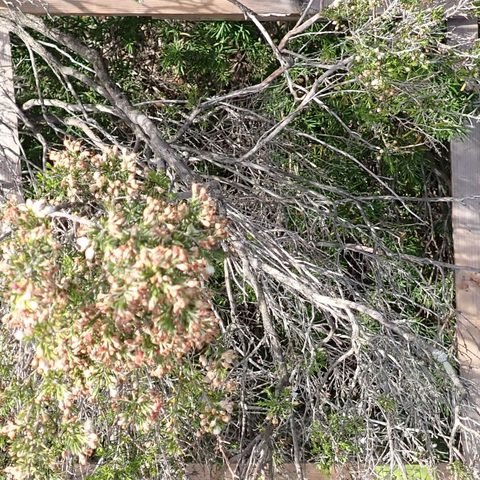
\includegraphics[width=\cellw, height=\cellh, keepaspectratio]{images/quadrats/GUARDEN-CBNMed-10-1-16-34-20240429.jpg}};

% ── Row 2 ──────────────────────────────────────────────────────────────
\node[label, below=\rowsep of i1.south] (l4) {LISAH-JAS-0-1-20220505.jpg};
\node[below=1mm of l4]                  (i4) {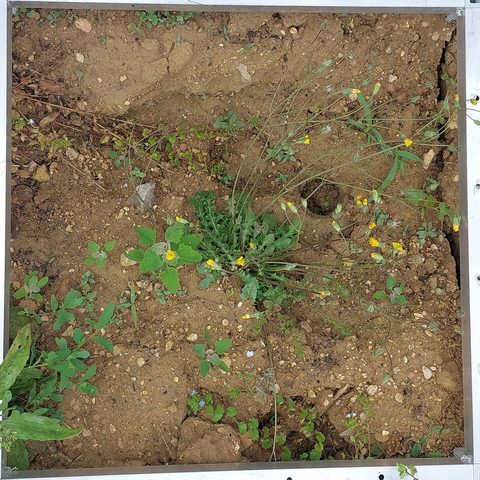
\includegraphics[width=\cellw, height=\cellh, keepaspectratio]{images/quadrats/LISAH-JAS-0-1-20220505.jpg}};

\node[label, right=\colsep of l4.east, anchor=west] (l5) {OPTMix-0108-P1-312-20231006.jpg};
\node[below=1mm of l5]                              (i5) {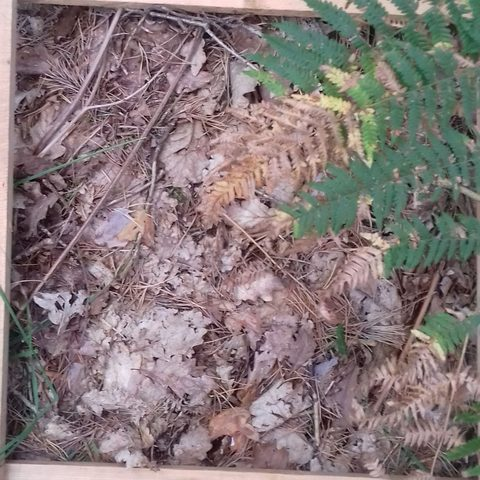
\includegraphics[width=\cellw, height=\cellh, keepaspectratio]{images/quadrats/OPTMix-0108-P1-312-20231006.jpg}};

\node[label, right=\colsep of l5.east, anchor=west] (l6) {RNNB-1-1-20230512.jpg};
\node[below=1mm of l6]                              (i6) {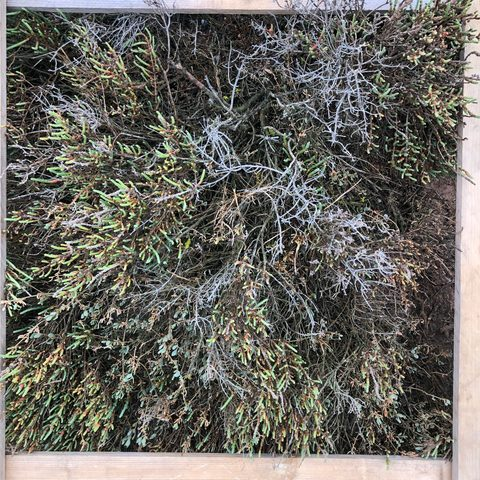
\includegraphics[width=\cellw, height=\cellh, keepaspectratio]{images/quadrats/RNNB-1-1-20230512.jpg}};

\end{tikzpicture}
